\documentclass[../Kamil_Kowalewski_Main.tex]{subfiles}

\begin{document} {

    Do eksperymentów został wykorzystany zbiór przedstawiony w~sekcji
    \ref{chapter4:srodowisko_eksperymentalne:zbiory_danych:1}

    \begin{table}[H]
        \scriptsize
        \centering
        \begin{tabularx}{\linewidth}{|L|c|c|c|c|}
            \hline
            % @formatter:off
            Nazwa & Eksperyment \#1 & Eksperyment \#2 & Eksperyment \#3 & Eksperyment \#4 \\ \hline
            Nazwa algorytmu & KMeansEvaluator & FuzzyCMeansEvaluator & BenchmarkEvaluator & BenchmarkEvaluator \\ \hline
            Czas wykonania (s) & 6.125 & 2.485 & 2.422 & 2.328 \\ \hline
            Liczba ofert określona jako wiarygodne & 5 & 5 & 6 & 4 \\ \hline
            Liczba ofert określona jako niewiarogodne & 6 & 6 & 5 & 7 \\ \hline
            % @formatter:on
        \end{tabularx}
        \caption
        [Statystyki dla zbioru danych \#1]
        {Statystyki dla zbioru danych \#1}
    \end{table}

    \begin{figure}[H]
        \centering
        \begin{minipage}[b]{0.49\textwidth}
            \centering
            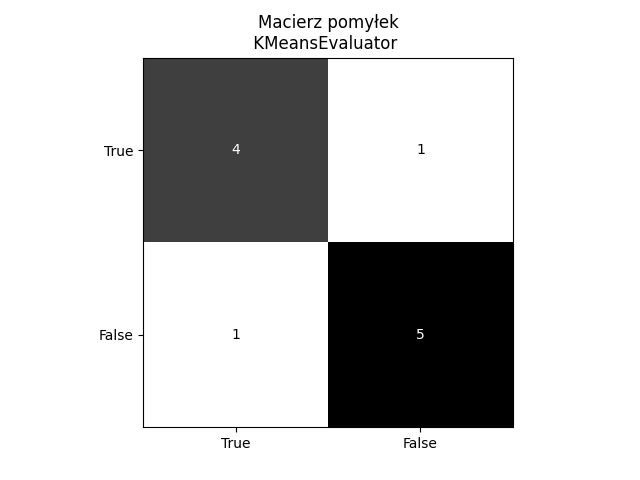
\includegraphics
            [width=\textwidth,keepaspectratio]
            {img/chapter5/dataset1/Logitechm330silentpluswirelessmouse_KMeansEvaluator.png}
            \caption
            [Macierz pomyłek dla zbioru danych \#1, eksperyment \#1]
            {Macierz pomyłek dla zbioru danych \#1, eksperyment \#1}
            \label{fig:chapter5:eksperymenty:zbior:1:eksperyment:1:macierz}
        \end{minipage}
        \hfill
        \begin{minipage}[b]{0.49\textwidth}
            \centering
            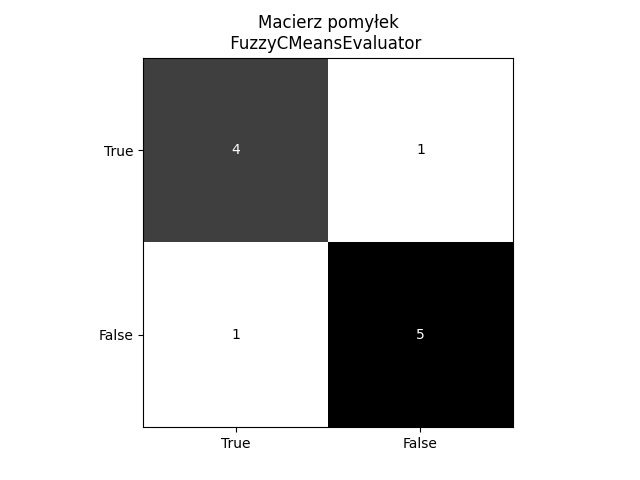
\includegraphics
            [width=\textwidth,keepaspectratio]
            {img/chapter5/dataset1/Logitechm330silentpluswirelessmouse_FuzzyCMeansEvaluator.png}
            \caption
            [Macierz pomyłek dla zbioru danych \#1, eksperyment \#2]
            {Macierz pomyłek dla zbioru danych \#1, eksperyment \#2}
            \label{fig:chapter5:eksperymenty:zbior:1:eksperyment:2:macierz}
        \end{minipage}
    \end{figure}

    \begin{figure}[H]
        \centering
        \begin{minipage}[b]{0.49\textwidth}
            \centering
            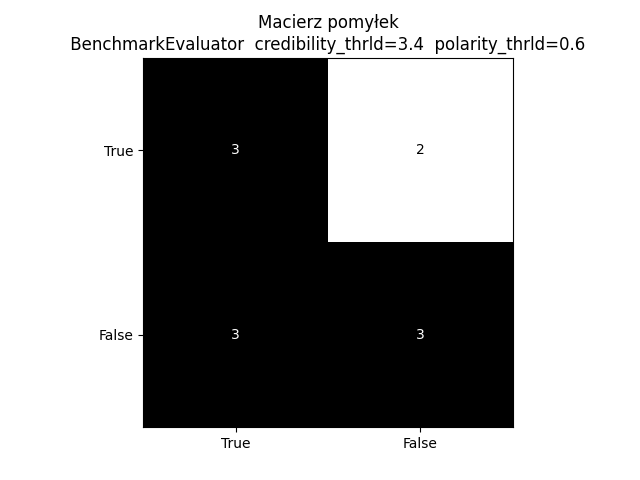
\includegraphics
            [width=\textwidth,keepaspectratio]
            {img/chapter5/dataset1/Logitechm330silentpluswirelessmouse_BenchmarkEvaluator.png}
            \caption
            [Macierz pomyłek dla zbioru danych \#1, eksperyment \#3]
            {Macierz pomyłek dla zbioru danych \#1, eksperyment \#3}
            \label{fig:chapter5:eksperymenty:zbior:1:eksperyment:3:macierz}
        \end{minipage}
        \hfill
        \begin{minipage}[b]{0.49\textwidth}
            \centering
            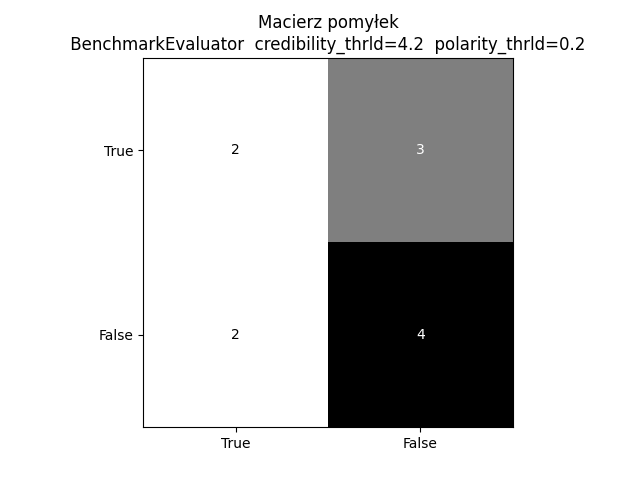
\includegraphics
            [width=\textwidth,keepaspectratio]
            {img/chapter5/dataset1/Logitechm330silentpluswirelessmouse_BenchmarkEvaluator-1.png}
            \caption
            [Macierz pomyłek dla zbioru danych \#1, eksperyment \#4]
            {Macierz pomyłek dla zbioru danych \#1, eksperyment \#4}
            \label{fig:chapter5:eksperymenty:zbior:1:eksperyment:4:macierz}
        \end{minipage}
    \end{figure}

    \subsection{Podsumowanie uzyskanych wyników}
    \label{chapter5:eksperymenty:zbior:1:podsumowanie} {
        Na podstawie powyższych wyników można stwierdzić, że dla tego zbioru danych
        najlepiej sprawdziła się autorska metoda, te same wyniki zostały uzyskane dla
        obu wariantów. Metody popełniły 2~błędy po jednym pierwszego i~drugiego
        rodzaju. Czas wykonania był dla wariantu K-Means był znacznie wyższy niż dla
        C-Means.

        W~przypadku metoda literaturowej to dla obu zestawów parametrów czasy wykonania
        były bardzo zbliżone. Jeżeli chodzi o~wyniki to w~eksperymencie \#3 metoda
        popełniła 2~błędy pierwszego rodzaju i~3~błędy drugiego rodzaju natomiast
        w~eksperymencie \#4 metoda popełniła 3~błędy pierwszego rodzaju i~2~błędy
        drugiego rodzaju. Można stwierdzić, że skuteczność autorskiej metody jest
        akceptowalna.
    }

}
\end{document}
